\chapter{Other SUSY results}
\label{chap:summary_susy}

In this chapter we discuss the interplay of the searched presented in the previous two chapters and the 
wide program of \gls{susy} searched carried on by the \gls{atlas} and \gls{cms} collaborations. 

\section{Gluino pair production}

\begin{figure}[htbp]
	\centering
	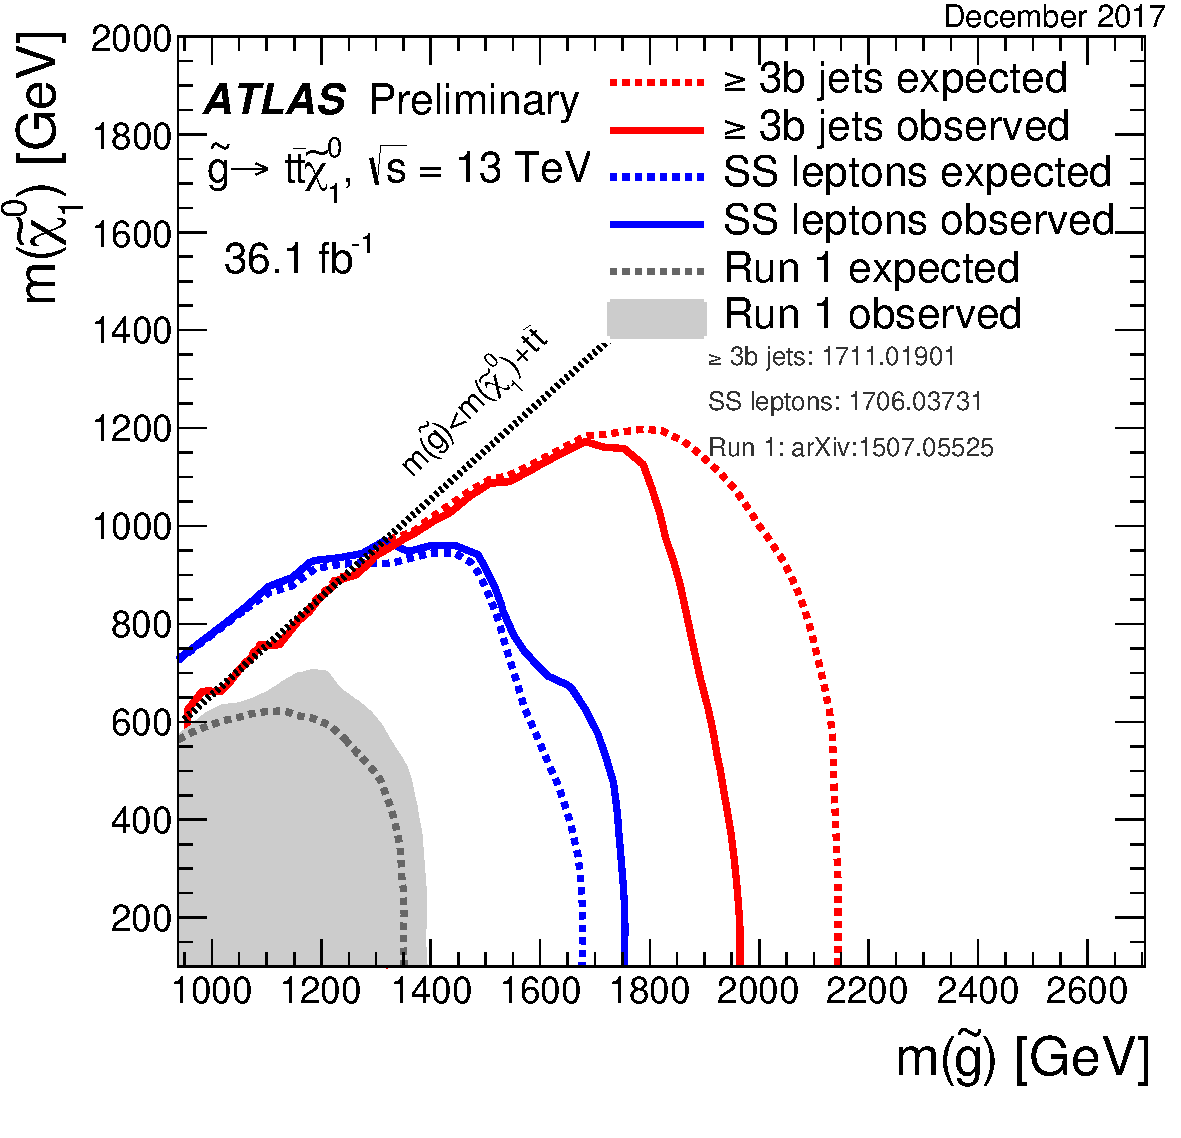
\includegraphics[width=0.65\textwidth]{figures/summary_plots/ATLAS_SUSY_Gtt.pdf}
	\caption{Exclusion limits at 95\% CL based on 13 TeV data in the (gluino, lightest neutralino) 
	mass plane for the Gtt simplified model where a pair of gluinos decays promptly via off-shell top 
	squarks to four top quarks and two lightest neutralinos. Theoretical signal cross section uncertainties are 
	not included in the limits shown. Figure from Ref. \cite{atlasSUSYSummary}.
	} 
	\label{fig:summary_atlas_Gtt}
\end{figure}

\begin{figure}[htbp]
	\centering 
	\subfigure[]{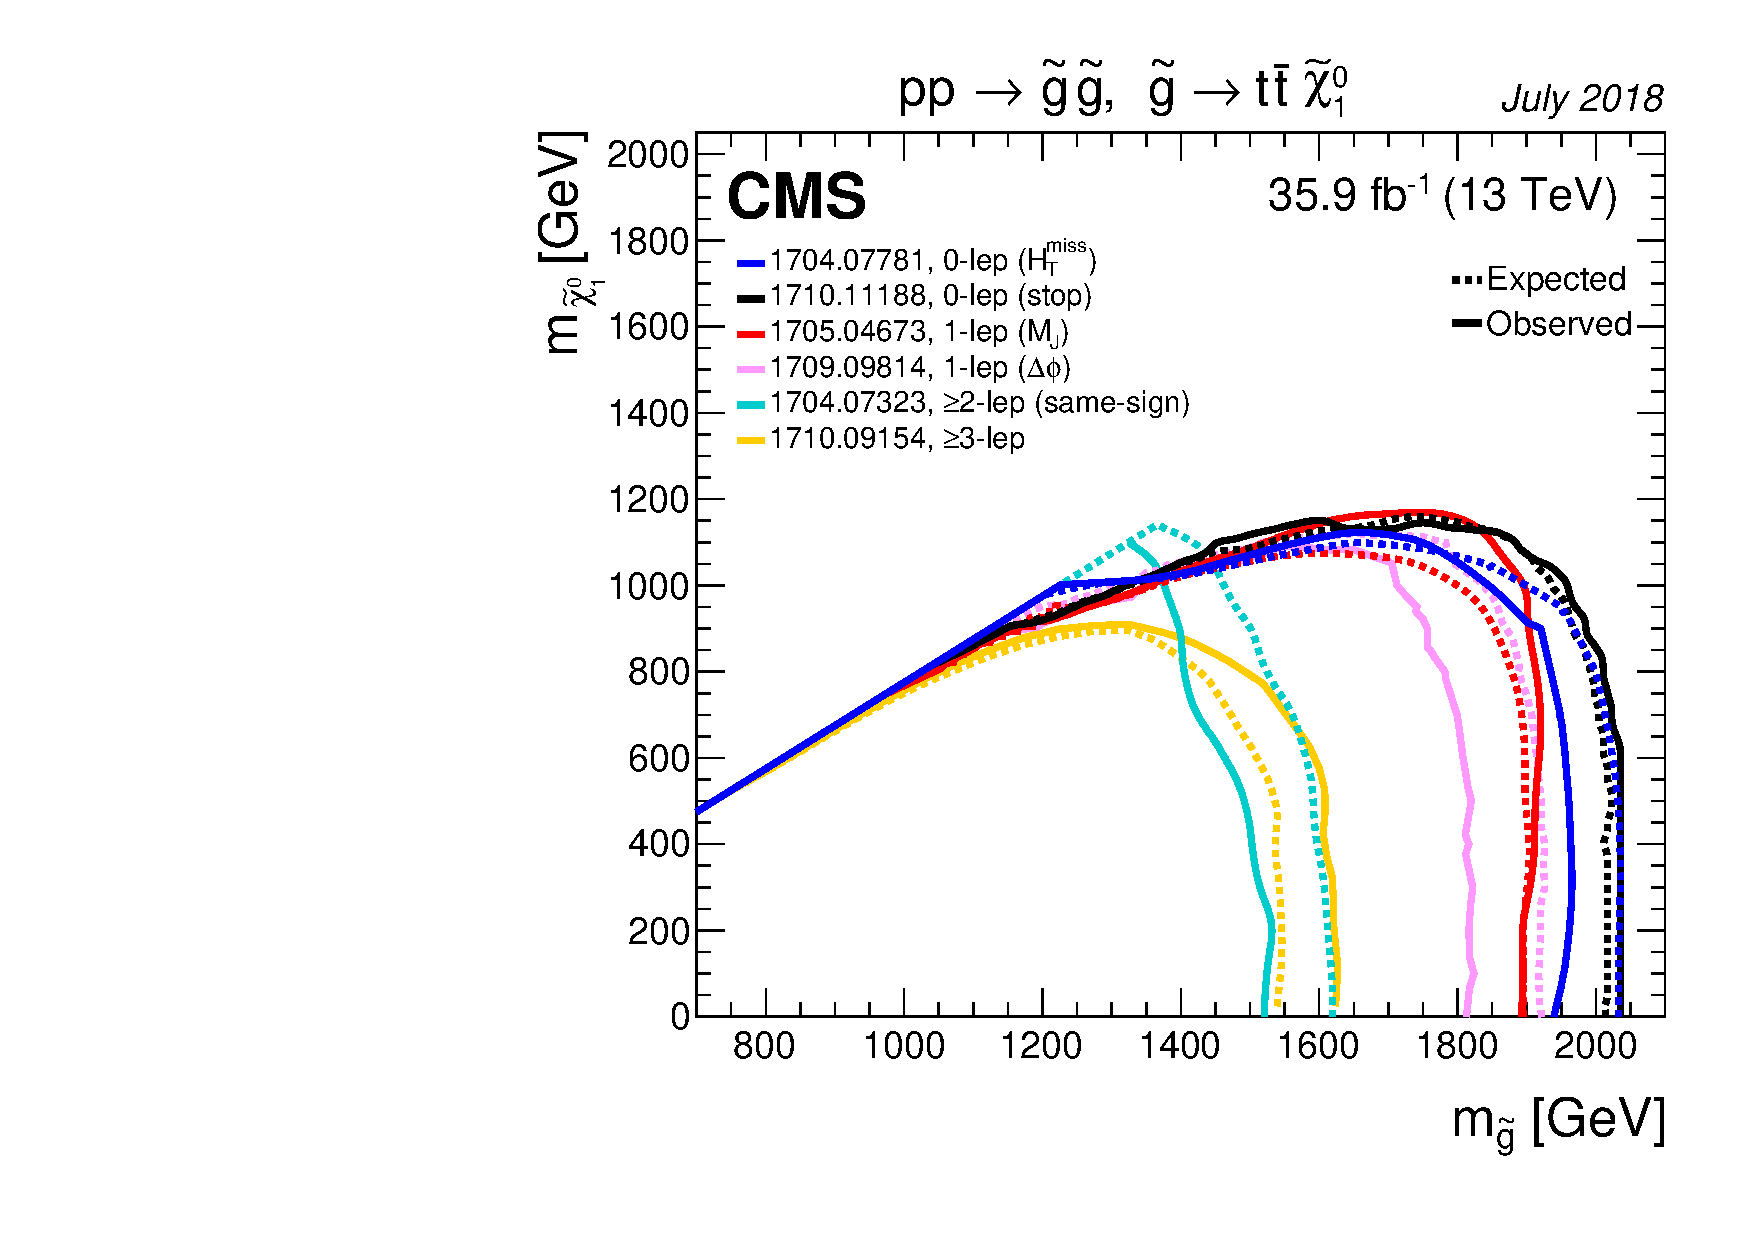
\includegraphics[width=0.49\textwidth]{figures/cms/T1tttt_limits_summary_cms.pdf}\label{fig:limits_Gtt_cms}}
	\subfigure[]{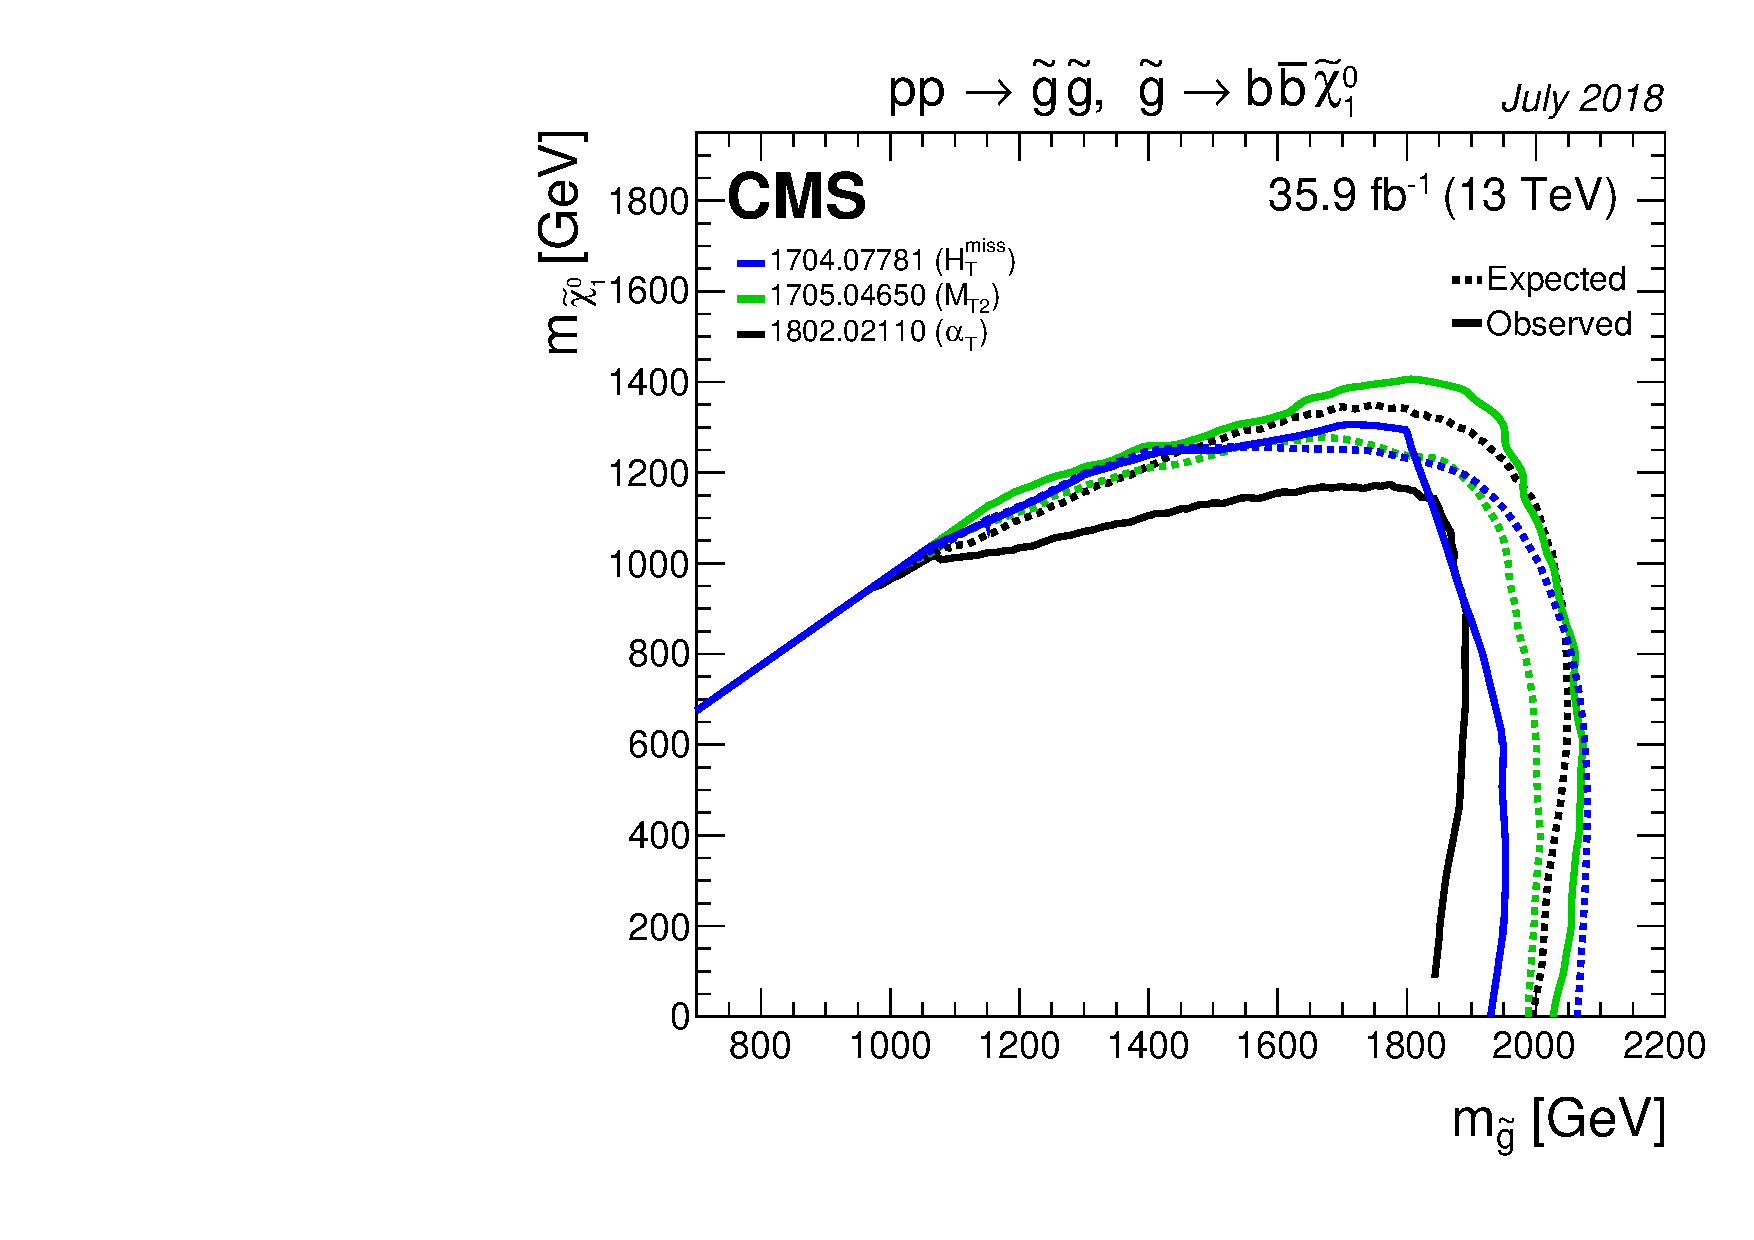
\includegraphics[width=0.49\textwidth]{figures/cms/T1bbbb_limits_summary_cms.pdf}\label{fig:limits_Gbb_cms}}
	\caption{Mass limits at 95\% CL obtained for simplified models of gluino pair production 
	with gluino decays to \subref{fig:limits_Gtt_cms} pairs of top quarks and the LSP and \subref{fig:limits_Gbb_cms}
	pairs of bottom quarks and the LSP. 
	In the figures, the solid (dashed) 
	lines correspond to the observed (median expected) limits. The arXiv numbers corresponding to the different analyses are shown in the legend.
	}
	\label{fig:limits_GbbGtt_comp}
\end{figure}

\FloatBarrier

\section{RPV interpretation}

\FloatBarrier

\section{Higgsino pair production in GMSB models}

The exclusion contours in the plane of m(\ninoone) \gls{br} plane are shown in Figures \ref{fig:summary_atlas_higgsino_GMSB} 
and \ref{fig:limits_higgsino_cms} for the \gls{atlas} and \gls{cms} collaborations respectively.

\begin{figure}[htbp]
	\centering
	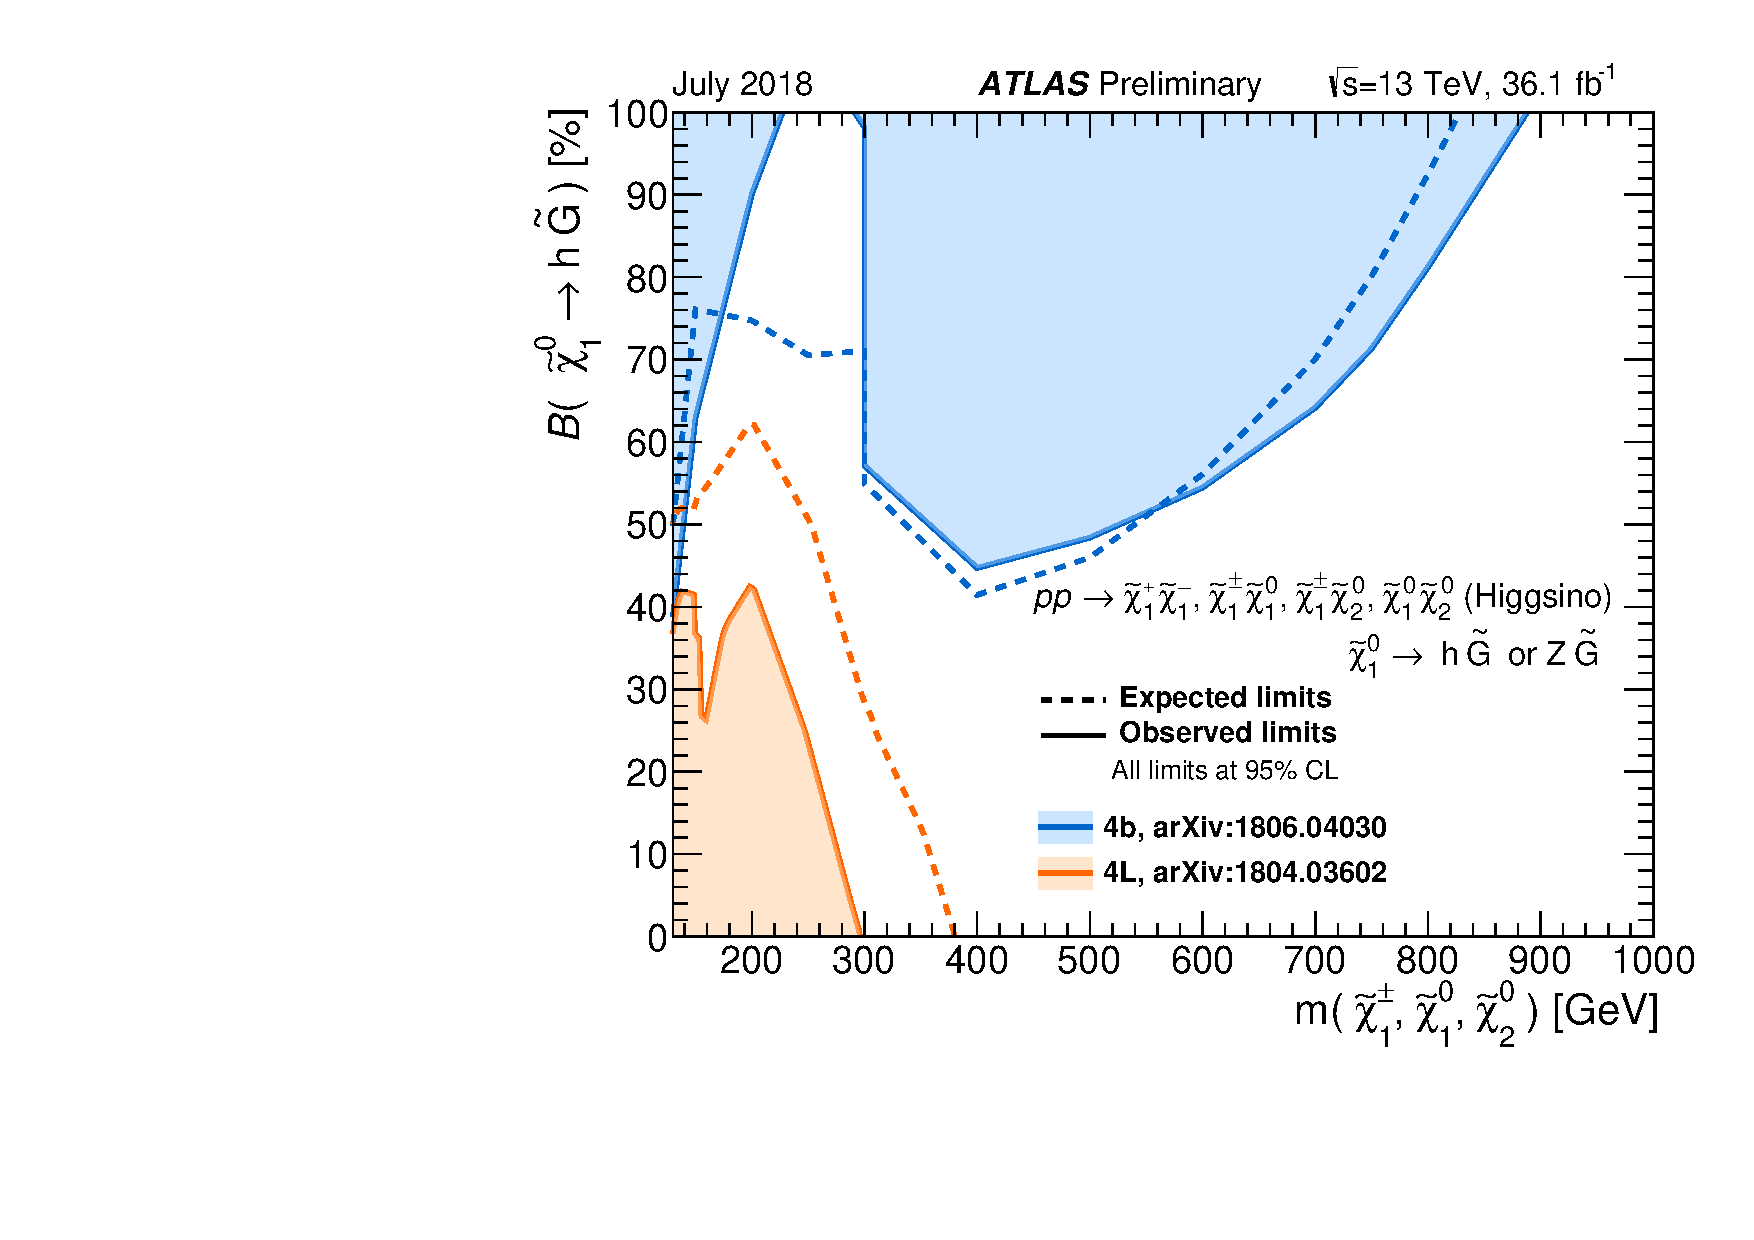
\includegraphics[width=0.65\textwidth]{figures/summary_plots/ATLAS_SUSY_EWSummary_GGM.pdf}
	\caption{The 95\% CL exclusion limits on a general gauge mediation model from 13 TeV data. 
	The model assumes a pure Higgsino NLSP that promptly decays to either Z gravitino or Higgs gravitino. 
	The limits are displayed as a function of the mass of the nearly mass-degenerate Higgsino triplet and the branching fraction of lightest Higgsino to Higgs gravitino. 	Figure from Ref. \cite{atlasSUSYSummary}.
	} 
	\label{fig:summary_atlas_higgsino_GMSB}
\end{figure}


\begin{figure}[htbp]
	\centering 
	\subfigure[]{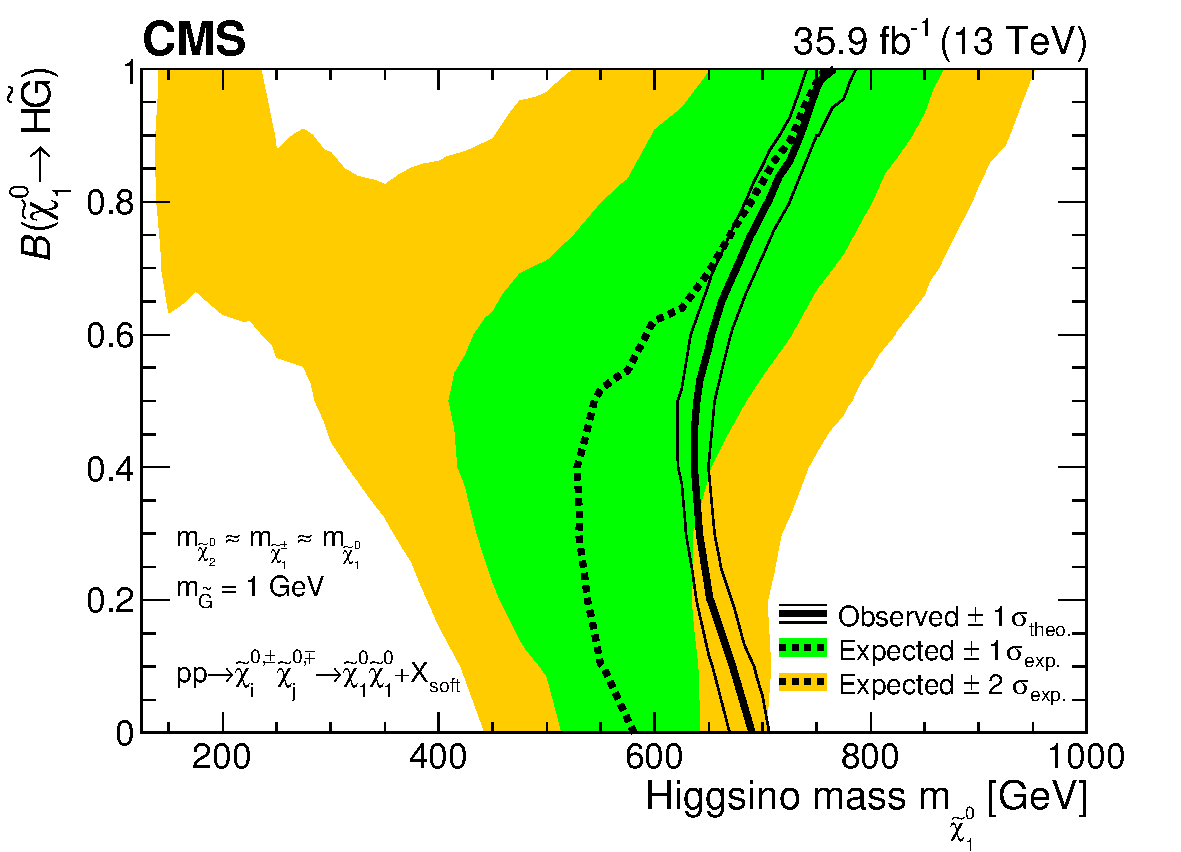
\includegraphics[width=0.49\textwidth]{figures/cms/CMS-SUS-17-004_Figure_011.pdf}\label{fig:limits_higgsino_cms_comb}}
	\subfigure[]{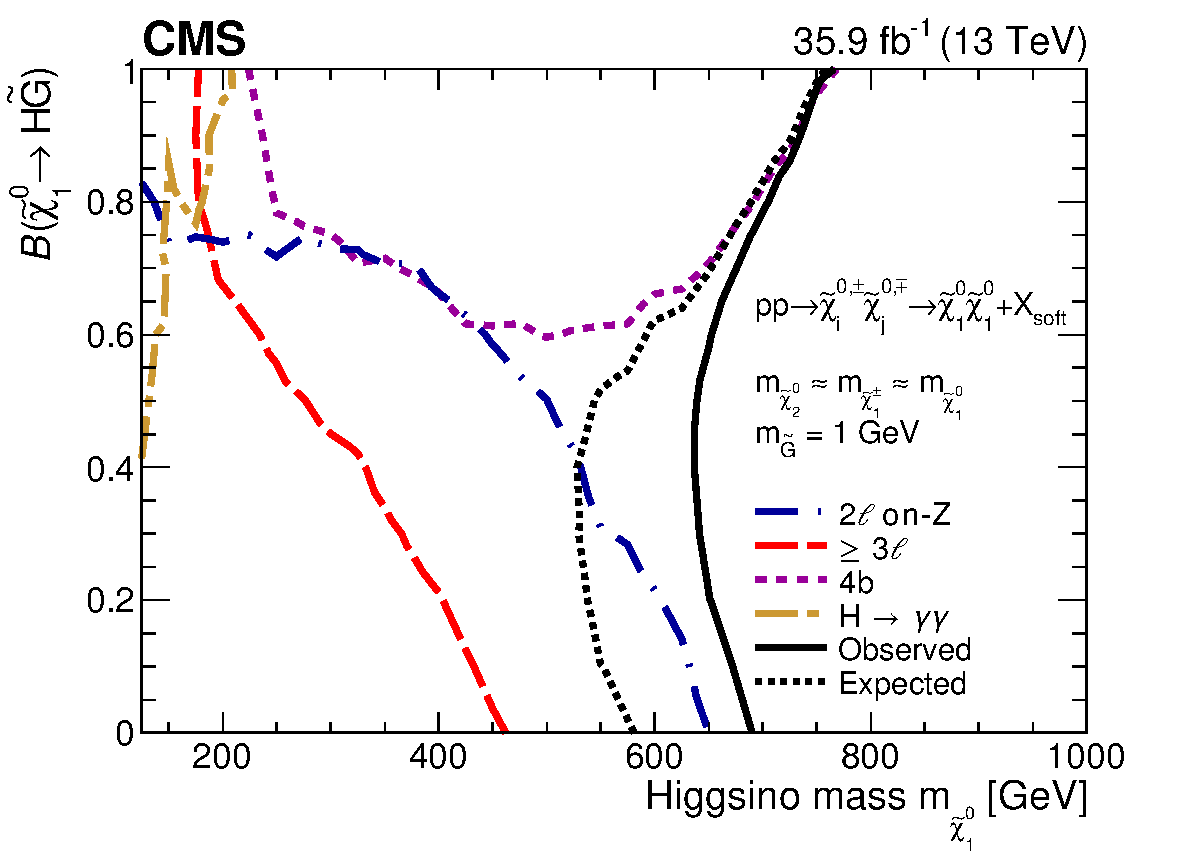
\includegraphics[width=0.49\textwidth]{figures/cms/CMS-SUS-17-004_Figure_012.pdf}\label{fig:limits_higgsino_cms_individual}}
	\caption{
	Exclusion contours at the 95\% CL in the plane of m(\ninoone) and \gls{br}(\ninoone $\to$ H \gravino) for the model of \ninoone\ninoone production.
    \subref{fig:limits_higgsino_cms_comb}     
	Combined exclusion contours. The area to the left of or below the solid (dashed) black curve represents the observed (expected) exclusion region. The green and yellow bands indicate the $\pm1$ and $2\sigma$ uncertainties in the expected limit. The thin black lines show the effect of the theoretical uncertainties ($\pm1\sigma_{theory}$) on the signal cross section.
	\subref{fig:limits_higgsino_cmsindividual}
	Observed contours for each individual analysis compared with the combination. For the 4b contour, the region above is excluded, while for all others, the region to the left is excluded. The 4b search drives the exclusion at large values of \gls{br}(\ninoone $\to$ H \gravino) while the on-Z dilepton and multilepton searches are competing at lower values of \gls{br}(\ninoone $\to$ H \gravino).
		}
	\label{fig:limits_higgsino_cms}
\end{figure}

\FloatBarrier


\section{Higgsino pair production in GMSB models}

\begin{figure}[htbp]
	\centering
	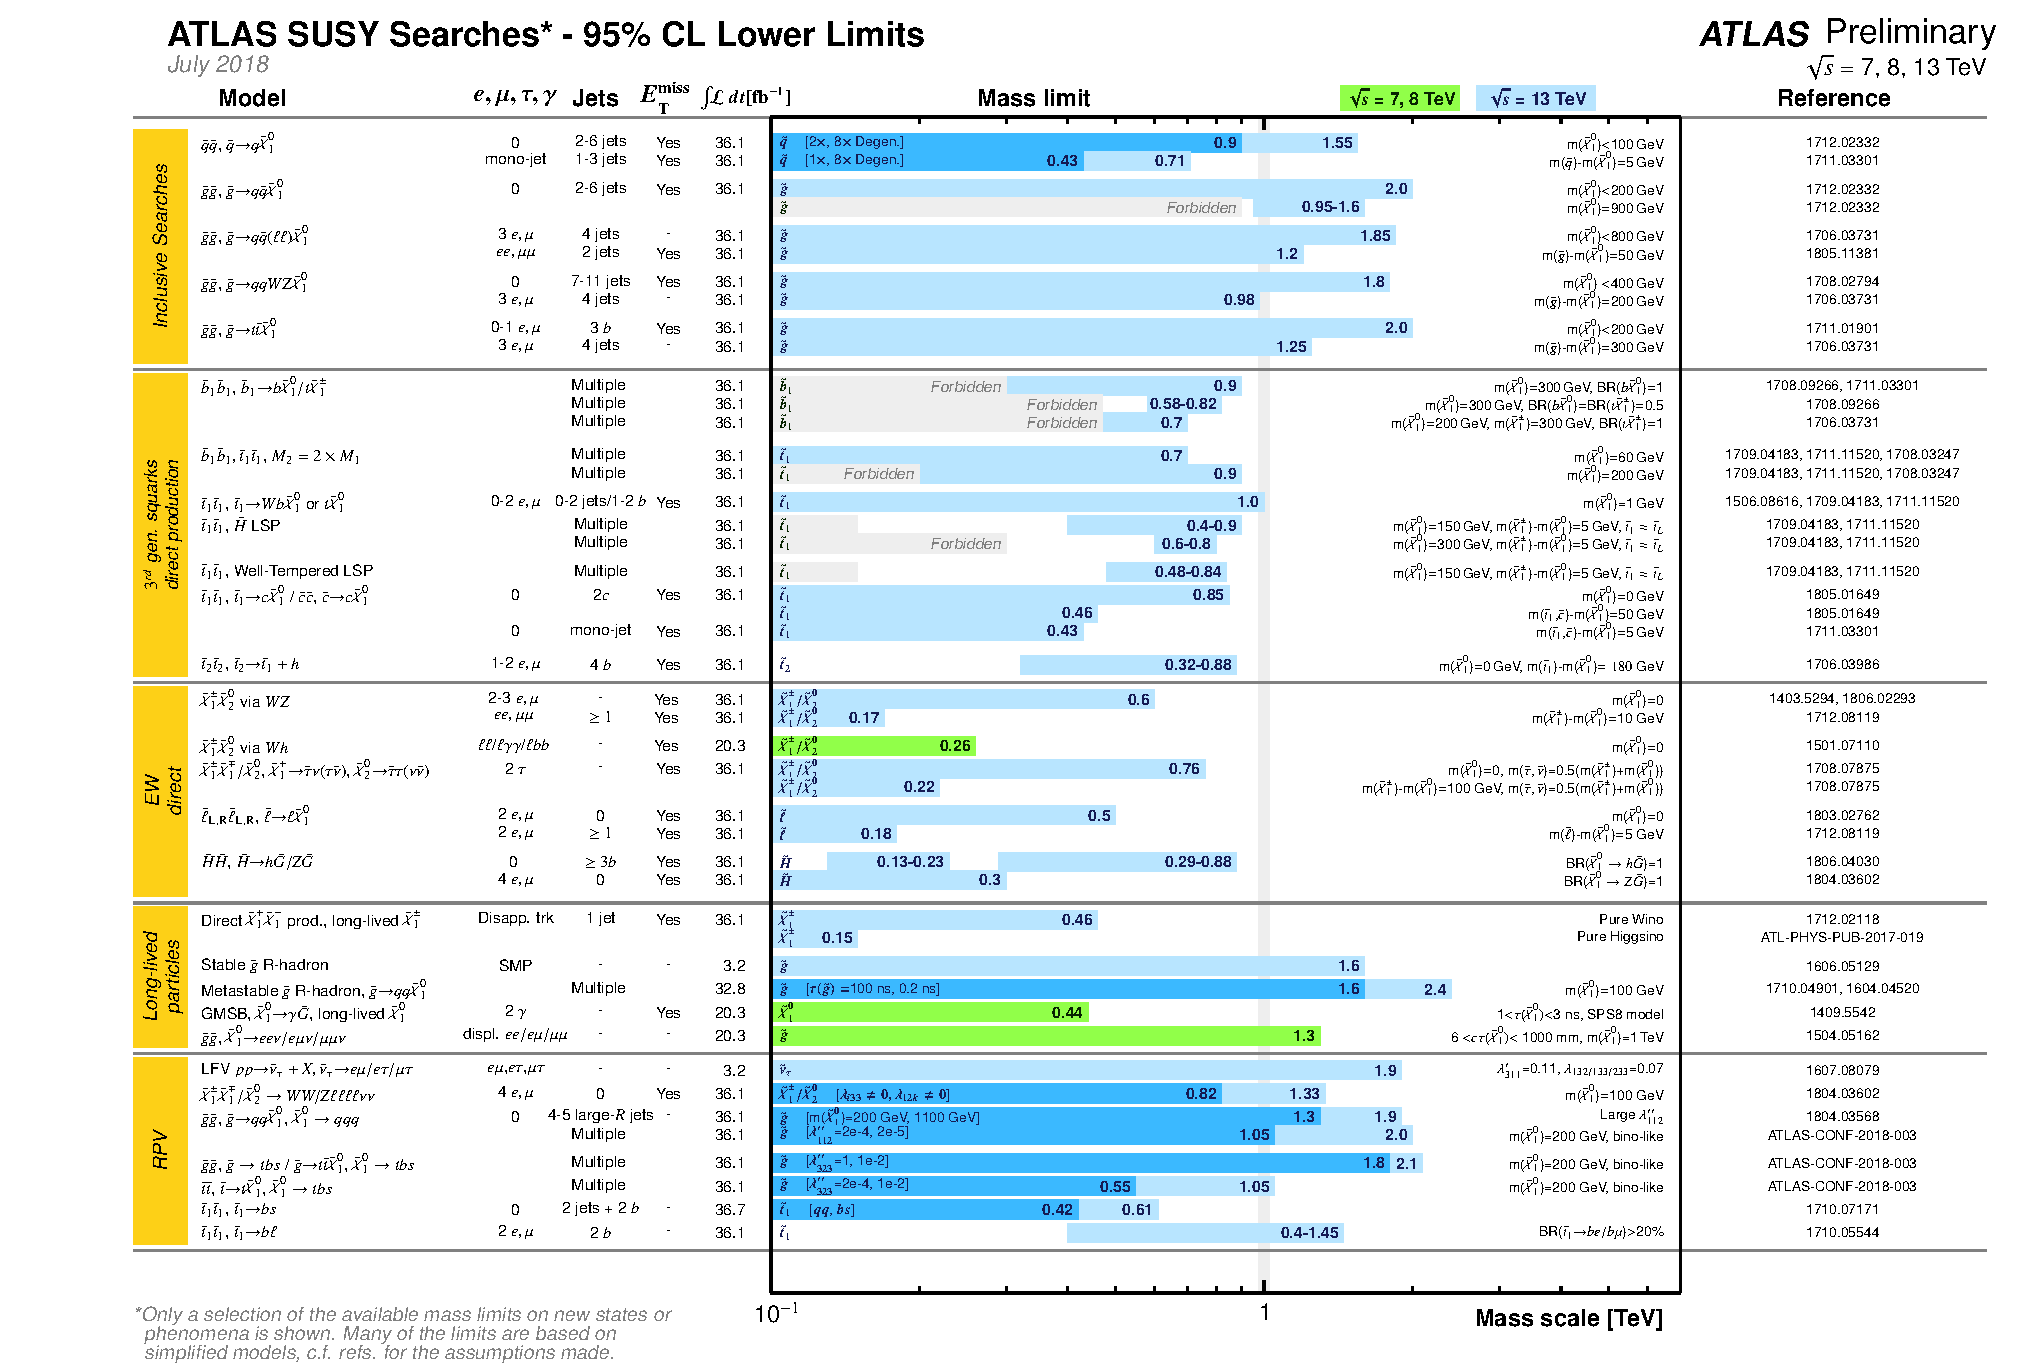
\includegraphics[width=1\textwidth]{figures/summary_plots/ATLAS_SUSY_Summary.pdf}
	\caption{	Mass reach of the ATLAS searches for Supersymmetry. 
	A representative selection of the available search results is shown. Results are quoted for the nominal cross section 
	in both a region of near-maximal mass reach and a demonstrative alternative scenario, in order to display the range in 
	model space of search sensitivity. Some limits depend on additional assumptions on the mass of the intermediate states, 
	as described in the references provided in the plot. Figure from Ref. \cite{atlasSUSYSummary}.
	} 
	\label{fig:summary_atlas_summary}
\end{figure}